\documentclass[12pt]{book}
\usepackage[utf8]{inputenc}
\usepackage[spanish]{babel}
\usepackage[backend=bibtex, sorting=none]{biblatex}
\bibliography{bibliografia}
\usepackage{graphics}
\usepackage{pst-all,pstricks-add,pst-math}
\usepackage{tikz}
\usepackage{float}
\usepackage{textcomp}
\usepackage{dsfont}
\usepackage{booktabs}
\usepackage{makeidx}
\usepackage[colorlinks=true, pdfborder={0 100 100}, linkcolor=orange, linktoc=page, citecolor=Green]{hyperref}
\usepackage{microtype}
\usepackage{amssymb}
\usepackage{amsmath}
\usepackage[format=hang, font=small, labelfont=bf, margin=1cm]{caption}


\definecolor{orange}{RGB}{250,120,0}
\definecolor{Green}{RGB}{50,200,100}

\renewcommand{\rmdefault}{phv} % Arial
\renewcommand{\sfdefault}{phv} % Arial
\renewcommand{\baselinestretch}{1.5}
\makeindex


\topmargin=0cm     %margen superior
\oddsidemargin=1.5cm  %margen izquierdx|o (por defecto queda a 1.5 cm)

\usepackage{multirow}
\setcounter{tocdepth}{4} 	%Inserta subsubsecciones y párrafos en el indice
\usepackage{cleveref}		%Inserta la palabra correspondiente al referenciar un objeto (Figura, Tabla, etc)
\crefname{equation}{ecuación}{ecuaciones}
\crefname{table}{tabla}{tablas}
\crefname{figure}{figura}{figuras}
\crefname{section}{sección}{Sección}
\crefname{chapter}{capítulo}{Capítulo}

\graphicspath{{Imagenes/}} 	%La carpeta de dibujos es figs
% \includeonly{Capitulo_02}	%Incluye sólo los archivos que se especifican como parámetro. Se mantiene numeración global del documento.


\begin{document}
\renewcommand{\contentsname}{Tabla de contenidos}	%Cambiar nombre de Índice por Tabla de contenidos
\renewcommand{\listfigurename}{Índice de Ilustraciones}	%Cambiar nombre de Índice de Figuras por Índice de Ilustraciones
\renewcommand{\indexname}{Índice analítico}		%Cambiar nombre de Índice alfabético -> Índice analítico
% \renewcommand{\figurename}{Índice de Ilustraciones}	%Cambiar nombre de Índice de Figuras por Índice de Ilustraciones
\renewcommand{\listtablename}{Índice de tablas}
\renewcommand{\tablename}{Tabla}

%%%%%%%%%%%%%%%%%%%%%%%%%%%%%%%%%%
%(1) PORTADA			[L]
%%%%%%%%%%%%%%%%%%%%%%%%%%%%%%%%%%
\begin{titlepage}
  \begin{flushright}
    \begin{tabular}{cl}
      &\multirow{4}{*}{\hspace{0cm}
\includegraphics[width=2cm]{logoBN.png}}\\
      \large{\textbf{UNIVERSIDAD DE SANTIAGO DE CHILE}}&  \\
      \textbf{FACULTAD DE CIENCIA}&\\
      \textbf{DEPARTAMENTO DE FÍSICA}& \\
    \end{tabular}
  \end{flushright}

\vspace*{3cm}

  \begin{center}
    \large{\textbf{SÍNTESIS DE GRAFENO Y SUPERCONDENSADORES BASADOS EN GRAFENO}}\\ %\vspace*{2cm}
  \end{center}
  \begin{center}
    \textbf{CARLOS JAVIER EUGENIO HERRERA}
  \end{center}

\vspace*{1cm}

  \begin{flushright}
    \begin{tabular}{ll}
      \textbf{Profesor Guía:}& DINESH PRATAP SINGH\\
    \end{tabular}
\\\vspace{3cm}

  \begin{center}
    \textbf{Trabajo de Titulación presentado en conformidad a los
    requisitos para obtener el título profesional de Ingeníero Físico.}
  \end{center}
  \end{flushright}

\vfill

  \begin{center}
    \textbf{Santiago -  Chile\\2016}
  \end{center}
\end{titlepage}

\newpage
\mbox{}
\thispagestyle{empty}
\pagenumbering{roman}

%%%%%%%%%%%%%%%%%%%%%%%%%%%%%%%%%%
%(2) DERECHOS DE AUTOR		[L]
%%%%%%%%%%%%%%%%%%%%%%%%%%%%%%%%%%
\vfill
\begin{center}
\textbf{© 2016, Carlos Eugenio\\
Algunos  derechos  reservados. 
Esta  obra  está  bajo  una  Licencia  Creative  Commons  Atribución-NoComercial-Compartir Igual  
3.0. Sus condiciones de uso pueden ser revisadas 
en: http://creativecommons.org/licenses/by-nc-sa/3.0/cl/.}
\\

\includegraphics[width=2cm]{by-nc-sa.png}
\end{center}

%%%%%%%%%%%%%%%%%%%%%%%%%%%%%%%%%%
%(3) HOJA DE CALIFICACIONES	[]
%%%%%%%%%%%%%%%%%%%%%%%%%%%%%%%%%%

%%%%%%%%%%%%%%%%%%%%%%%%%%%%%%%%%%
%(4) DEDICATORIA(OPTATIVA)	[]
%%%%%%%%%%%%%%%%%%%%%%%%%%%%%%%%%%
\newpage
\chapter*{}
\begin{flushright}
\textit{Dedicatoria}
\end{flushright}
\newpage

%%%%%%%%%%%%%%%%%%%%%%%%%%%%%%%%%%
%(5) AGRADECIMIENTOS(OPTATIVA)	[]
%%%%%%%%%%%%%%%%%%%%%%%%%%%%%%%%%%
\chapter*{Agradecimientos} % *si no queremos que añada la palabra "Capitulo"
% \addcontentsline{toc}{chapter}{Agradecimientos} % si queremos que aparezca en el índice


%%%%%%%%%%%%%%%%%%%%%%%%%%%%%%%%%%
%(6) TABLA DE CONTENIDOS 	[]
%%%%%%%%%%%%%%%%%%%%%%%%%%%%%%%%%%
\newpage
\tableofcontents
\newpage
\newrgbcolor{xdxdff}{0.49 0.49 1}
\newrgbcolor{ffqqtt}{1 0 0.2}
\psset{xunit=1.0cm,yunit=1.0cm,algebraic=true,dotstyle=*,dotsize=3pt
0,linewidth=0.8pt,arrowsize=3pt 2,arrowinset=0.25}

%%%%%%%%%%%%%%%%%%%%%%%%%%%%%%%%%%
%(7) ÍNDICE DE TABLAS		[]
%%%%%%%%%%%%%%%%%%%%%%%%%%%%%%%%%%
\newpage
\listoftables
\newrgbcolor{xdxdff}{0.49 0.49 1}
\newrgbcolor{ffqqtt}{1 0 0.2}
\psset{xunit=1.0cm,yunit=1.0cm,algebraic=true,dotstyle=*,dotsize=3pt
	0,linewidth=0.8pt,arrowsize=3pt 2,arrowinset=0.25}
%%%%%%%%%%%%%%%%%%%%%%%%%%%%%%%%%%
%(8) ÍNDICE DE ILUSTRACIONES	[]
\newpage
\listoffigures
\newrgbcolor{xdxdff}{0.49 0.49 1}
\newrgbcolor{ffqqtt}{1 0 0.2}
\psset{xunit=1.0cm,yunit=1.0cm,algebraic=true,dotstyle=*,dotsize=3pt
0,linewidth=0.8pt,arrowsize=3pt 2,arrowinset=0.25}
%%%%%%%%%%%%%%%%%%%%%%%%%%%%%%%%%%

%%%%%%%%%%%%%%%%%%%%%%%%%%%%%%%%%%
%(9) RESUMEN			[]
%%%%%%%%%%%%%%%%%%%%%%%%%%%%%%%%%%
\newpage
\chapter*{Resumen}
\addcontentsline{toc}{chapter}{Resumen} % si queremos que aparezca en el índice

\newpage
\pagenumbering{arabic}
%%%INTRODUCCIÓN GENERAL%%%
\chapter*{Introducción}
\addcontentsline{toc}{chapter}{Introducción}

El prefijo nano deriva del griego \emph{nanos}, que significa literalmente ``enano''. En el sistema internacional de unidades, el prefijo nano representa un factor de $\mathrm{10^{-9}}$, o una mil millonésima parte. Al añadir este prefijo a la unidad de longitud, obtenemos ``nanómetro'' (nm), o una mil millonésima parte de un metro. Así la nanotecnología es, a grandes rasgos, la ciencia, tecnología, e ingeniería que trata sistemas en el rango aproximado de 1-100 nanómetros. \citep{Haick2013,Gressler2013}. Se ha de tener claro en que rango de dimensiones se encuentra la escala nanométrica, los seres humanos estamos acostumbrados a escalas grandes, se nos hace fácil entender las comparaciones de kilómetros con metros, o milímetros con metros, pero al reducir el tamaño a micrómetros o nanómetros nos cuesta, pues son escalas que se escapan de nuestros sentidos. Para ponerlo en perspectiva, un nanómetro esa un metro como un metro es a un millón de kilómetros. La figura \ref{fig:scale} muestra una escala de tamaños con varios ejemplos desde la escala humana hasta la atómica, la nanoescala comprende aproximadamente desde los cientos de nanómetros hasta fracciones de nanómetros.

\begin{figure}[h!]
	\centering
	\fbox{
		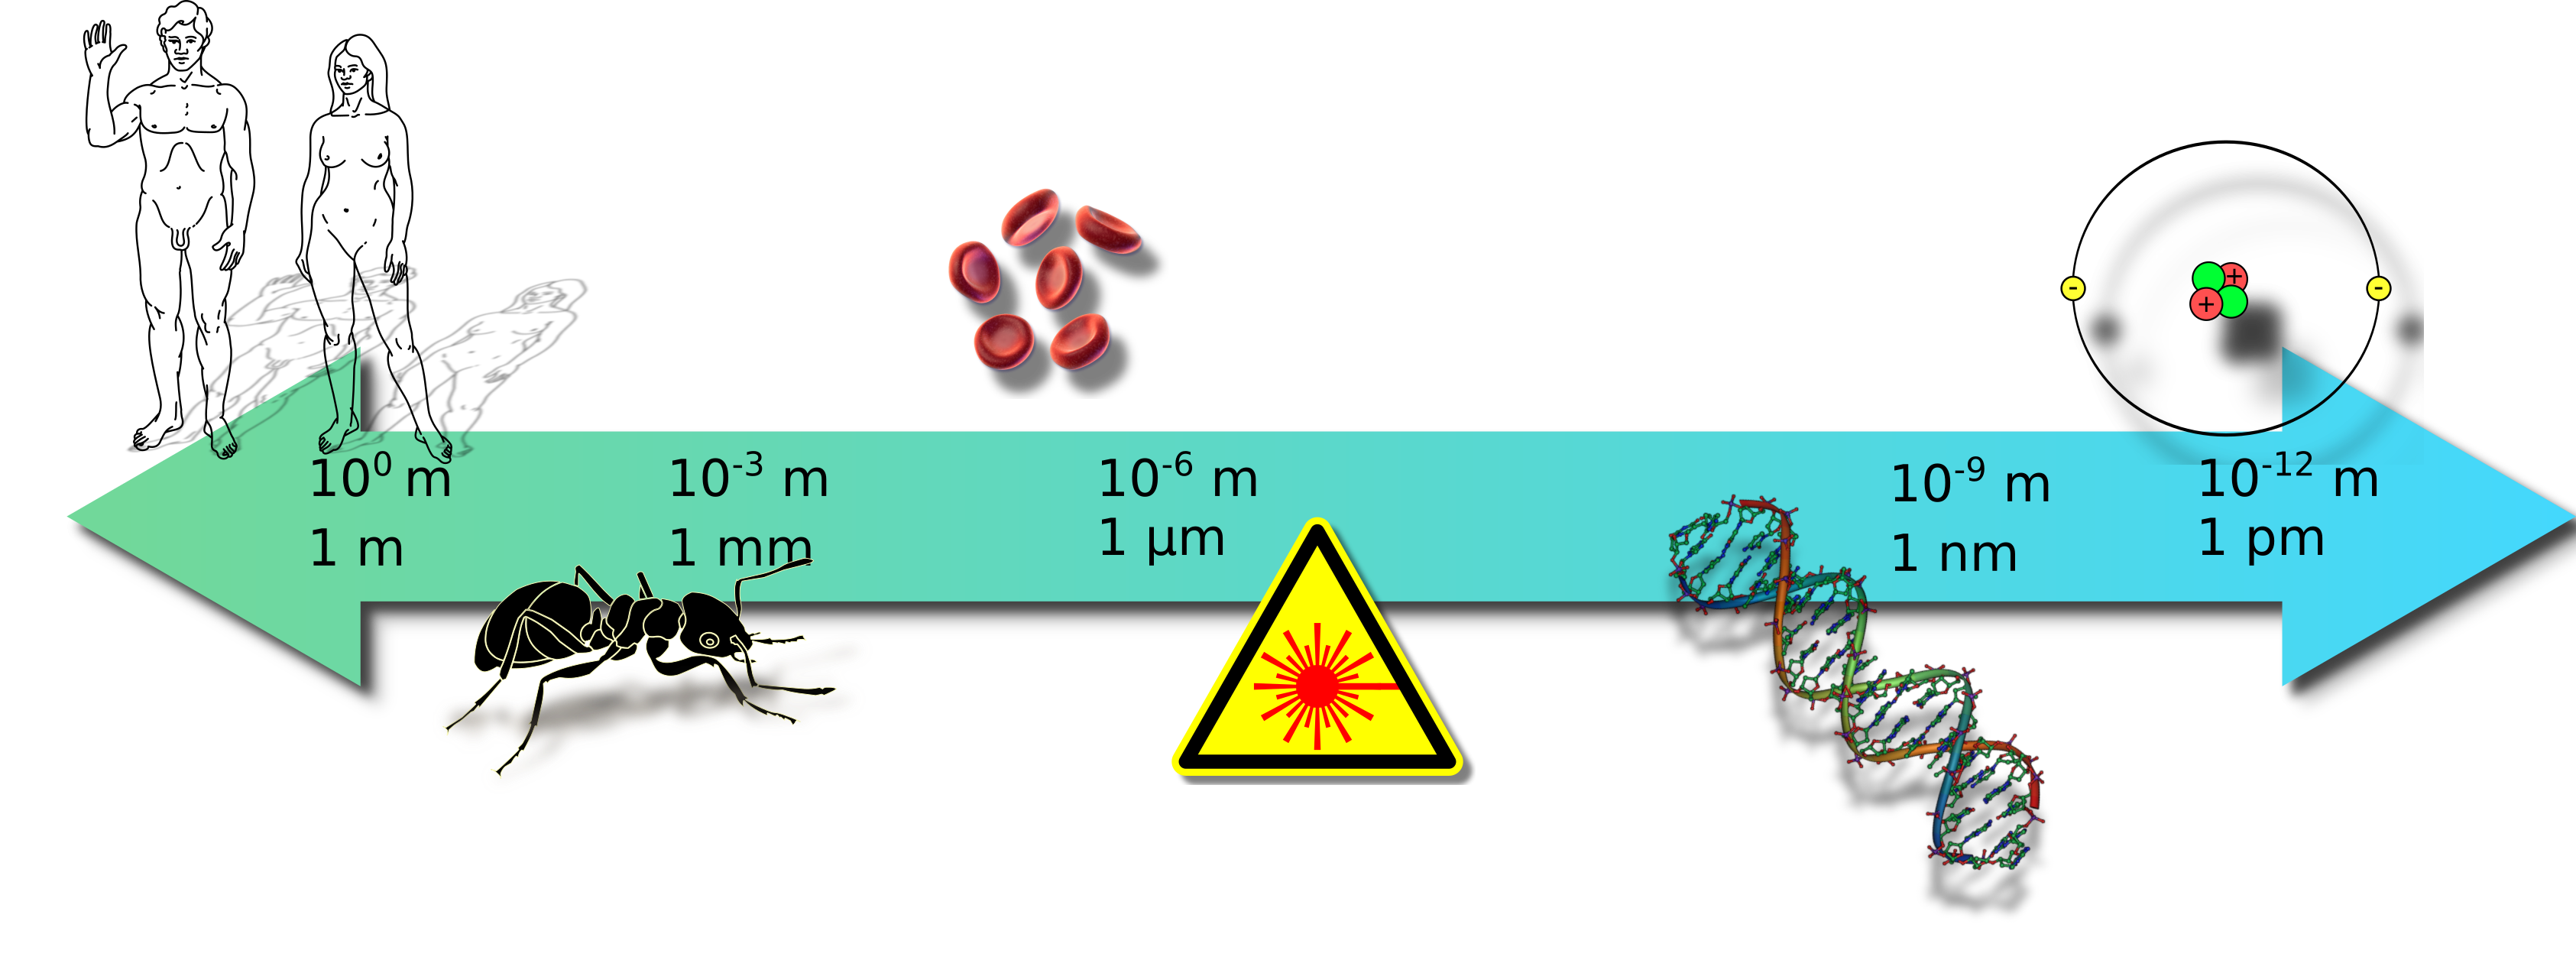
\includegraphics[width=\textwidth]{scale.png}
	}
	\caption[Comparativa de ódenes de magnitud desde metros hasta picometros]{Comparativa de órdenes de magnitud. De izquierda a derecha: Escala humana 1-2 m. Insectos 10 cm - 1 mm. Glóbulos rojos 6 $\mathrm{\mu}$m. Longitud de onda de luz visible 780-380 nm. Doble hélice de ADN 2 nm. Radio atómico de un átomo de helio 31 pm.}
\label{fig:scale}
\end{figure}

La idea de la nanotecnología fue vislumbrada por el físico Richard Feynman y expuesta en su charla \emph{``There is plenty room at the bottom''} \citep{Feynman1960}. Allí Feynman plantea que no existen barreras físicas que impidan manipular sistemas nanométricos, moléculas, o incluso átomos. La era moderna de la nanotecnología comienza con el desarrollo del microscopio de efecto túnel por Binning y Rohrer en 1981 \citep{Binnig1982}, que les hizo ganar el Premio Nobel de Física en 1986. Un microscopio de efecto túnel (STM por sus siglas en inglés \emph{Scanning Tunneling Microscope}), puede superar resoluciones de 0,1 nm de resolución lateral, y 0,01 nm en profundidad, y trabajar en variadas condiciones, sin necesidad de alto vacío o bajas temperaturas. Además de poder resolver átomos, el STM también puede manipularlos \citep{Chen2008}.

Una forma simple de clasificar los nanomateriales surge del número de dimensiones del material que no están en la nanoescala (ver figura \ref{fig:carbon_allotropes}). Un material que no posee ninguna dimensión en la nanoescala (material \emph{bulk}), se denomina material 3D y no  se considera un nanomaterial\footnote{A veces se les llama nanomateriales 3D a materiales formados por nanomateriales (2D, 1D, o 0D), que forman estructuras tridimensionales macroscópicas y muestran propiedades de nanomateriales, como por ejemplo, los aerogeles.}. Si una dimensión del material está en la nanoescala, se habla de material 2D, análogamente, con dos dimensiones en la nanoescala se trata de un nanomaterial 1D, y por último, si todas las dimensiones están en la nanoescala se denomina nanomaterial 0D.
\begin{figure}
	\centering
	\fbox{
		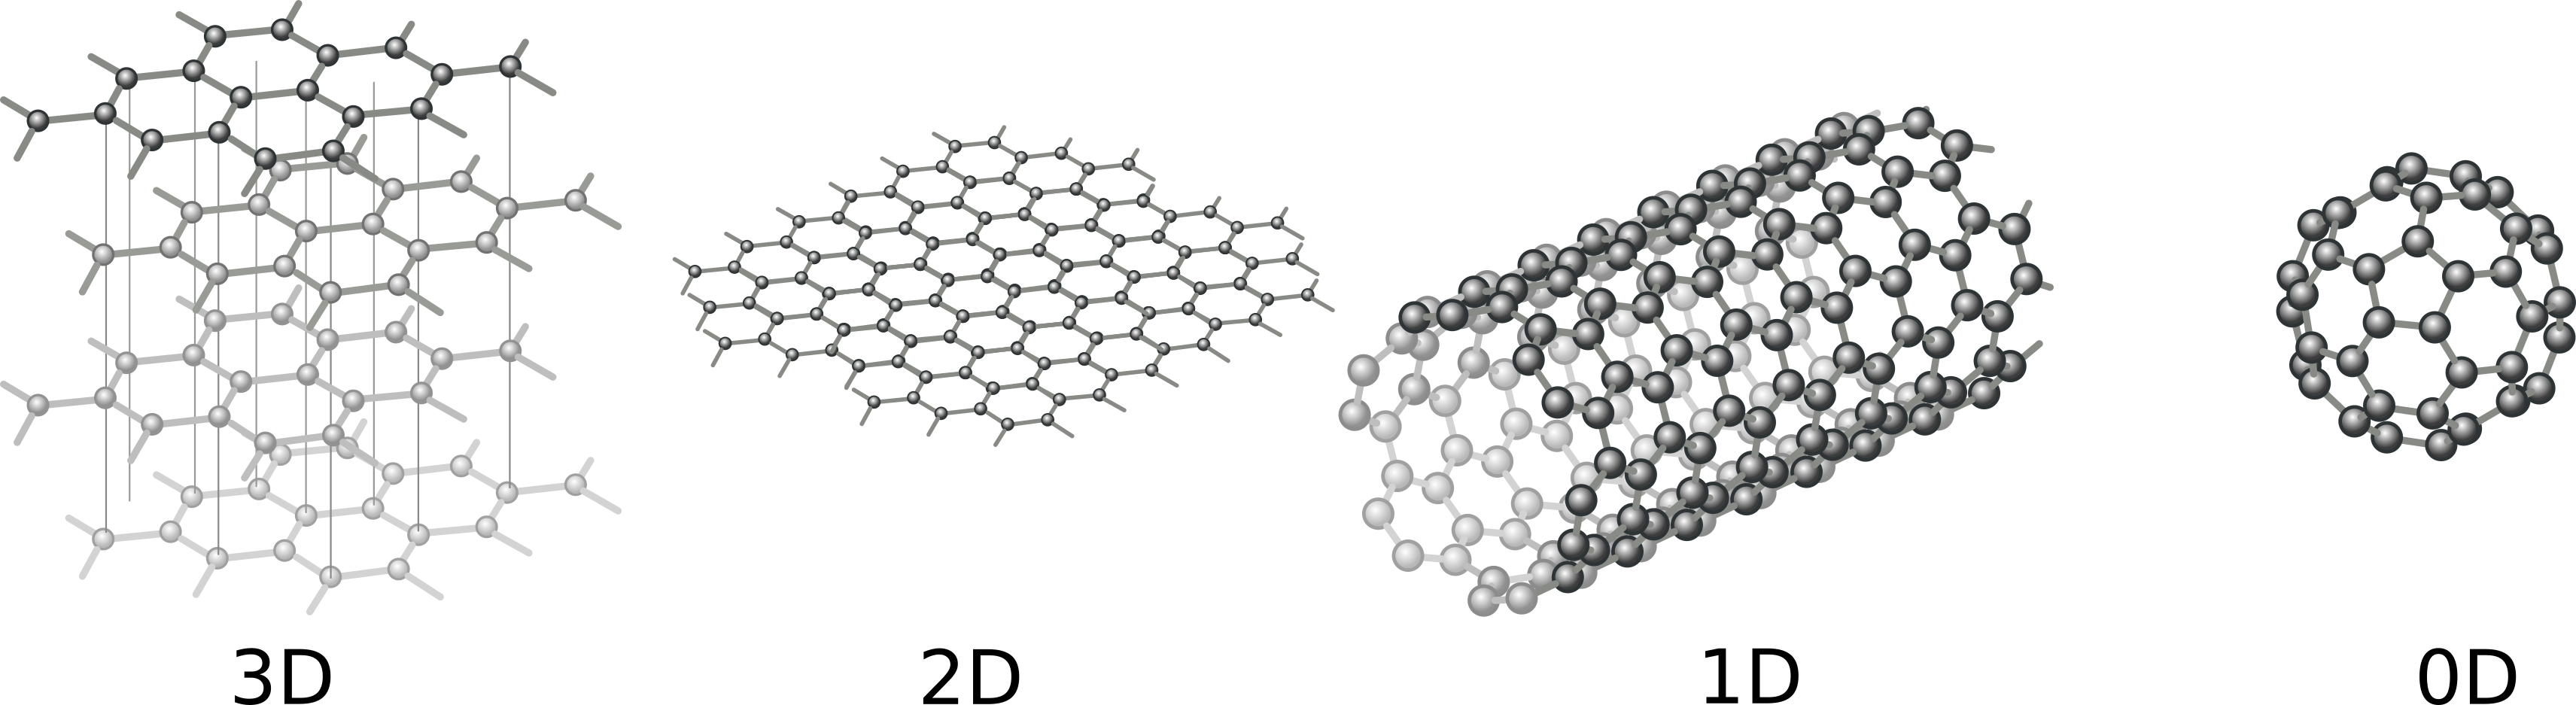
\includegraphics[width=\textwidth]{carbon_alotropes.png}
		}
	\caption[Alótropos del carbono mostrando las diferentes dimensionalidades de los nanomateriales]{Alótropos del carbono como representación de las diferentes dimensionalidades en los nanomateriales. De izquierda a derecha: Grafito, no es un material nanoestructurado, a pesar de estar formado por varios capas de grafeno. Grafeno, solo un átomo de espesor, es un material 2D. Nanotubo de carbono, es un material 1D. Fulereno, es un material 0D.}
	\label{fig:carbon_allotropes}
\end{figure}

\section*{La física de sistemas nanométricos}


%CONFINAMIENTO cuántico
Al reducir las dimensiones a escalas nanométricas, surgen efectos de confinamiento cuántico, pues se restringe el movimiento de los electrones en el material, esto conlleva a la discretización de los niveles de energía de los electrones y al cambio de la densidad de estados del material. 



%DENSIDAD de estados en diferentes dimensiones
Dependiendo de cuantas dimensiones son llevadas a la nanoescala, es como se ve afectada la densidad de estados.

\begin{figure}[h!]
	\centering
	\fbox{
		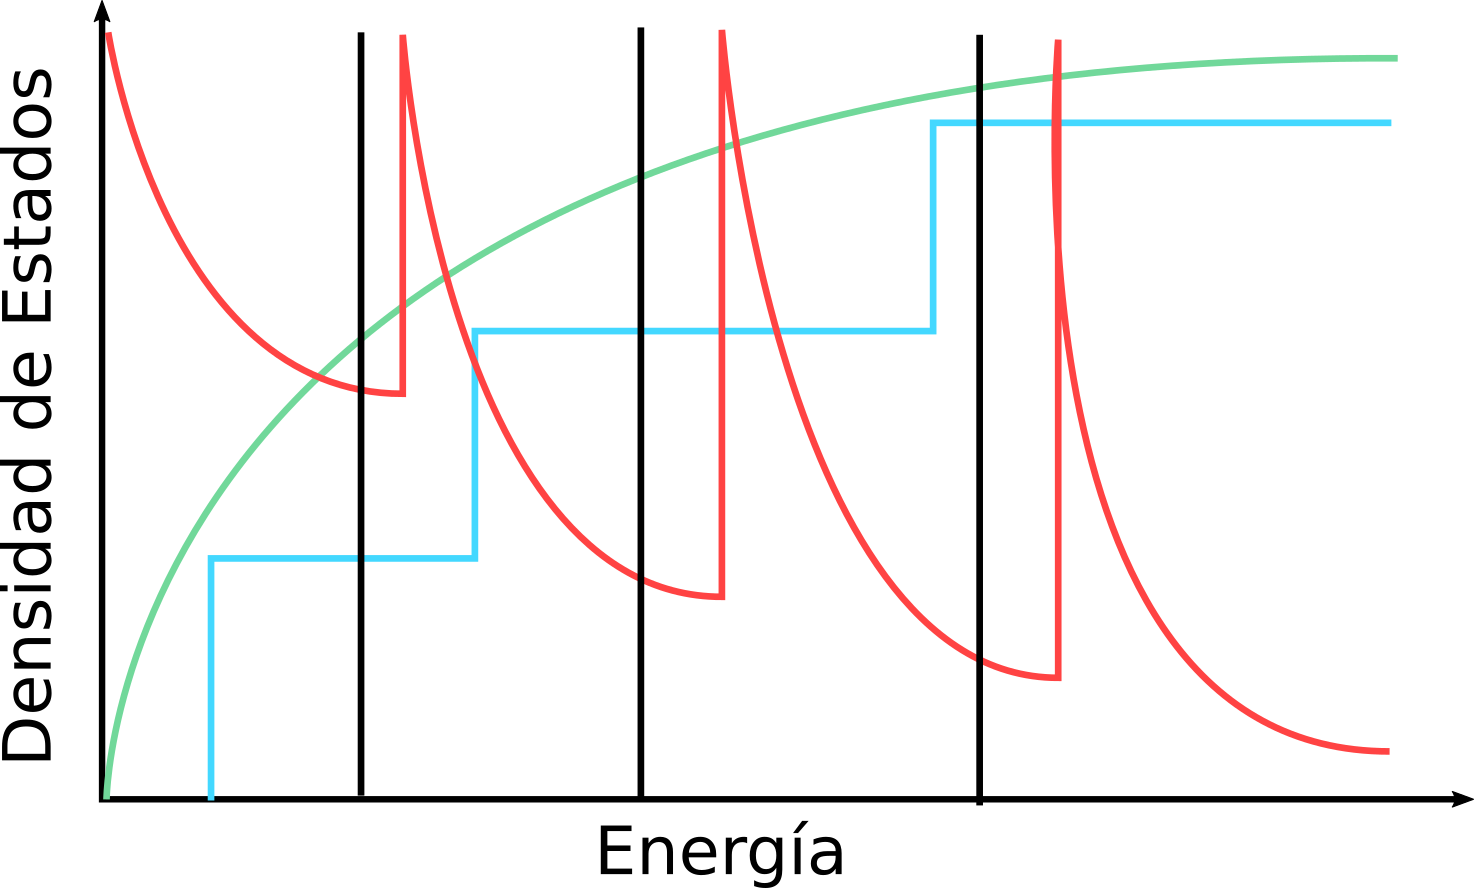
\includegraphics[width=0.6\textwidth]{DoE.png}
	}
	\caption[Densidad de estados en diferentes dimensionalidades]{Densidad de estados diferentes dimensiones. Para materiales 3D (no nanoestructurados), la densidad de estados es continua. En nanomateriales 2D, la densidad de estado forma escalones. Para materiales 1D, ésta es}
	\label{fig:DoE}
\end{figure}

%AREA superficial
Al dividir un volumen en partículas más pequeñas, el área superficial aumenta. Por ejemplo, en la secuencia de la figura \ref{fig:area_cubes}, el volumen total en cada división no cambia, pero el área superficial se dobla \footnotemark, siguiendo está lógica, al reducir un cubo de lado 1 cm a 100 nm, el área total habrá aumentado 100.000 veces. El aumento del área superficial aumenta la reactividad del material, ya que hay más lugar para, por ejemplo, reacciones químicas. Otra forma de verlo, es considerar la proporción de átomos en la superficie, con la cantidad de átomos del interior (proporción de área superficial al volumen), esta proporción aumenta al disminuir el tamaño de las partículas.

\footnotetext{Si en la secuencia de la figura \ref{fig:area_cubes} el cubo más grande tiene lado $l$, su área superficial es $6 \times l^2$, en la primera división, el lado de cada cubo es $l/2$ y el área de cada uno es $6\left( l/2\right)^2$, que en total hacen $6\left(l/2\right)^2\times 8$, en la segunda división el área total es $6\left(l/4\right)^2\times 8 \times 8$, así, en la n-ésima división el área es $6l^2 \left(1/2^n\right)^2\times 8^n$ o $6l^2 \times 2^n$. Así, el área superficial se dobla con cada división.}

\begin{figure}[h!]
	\centering
	\fbox{
		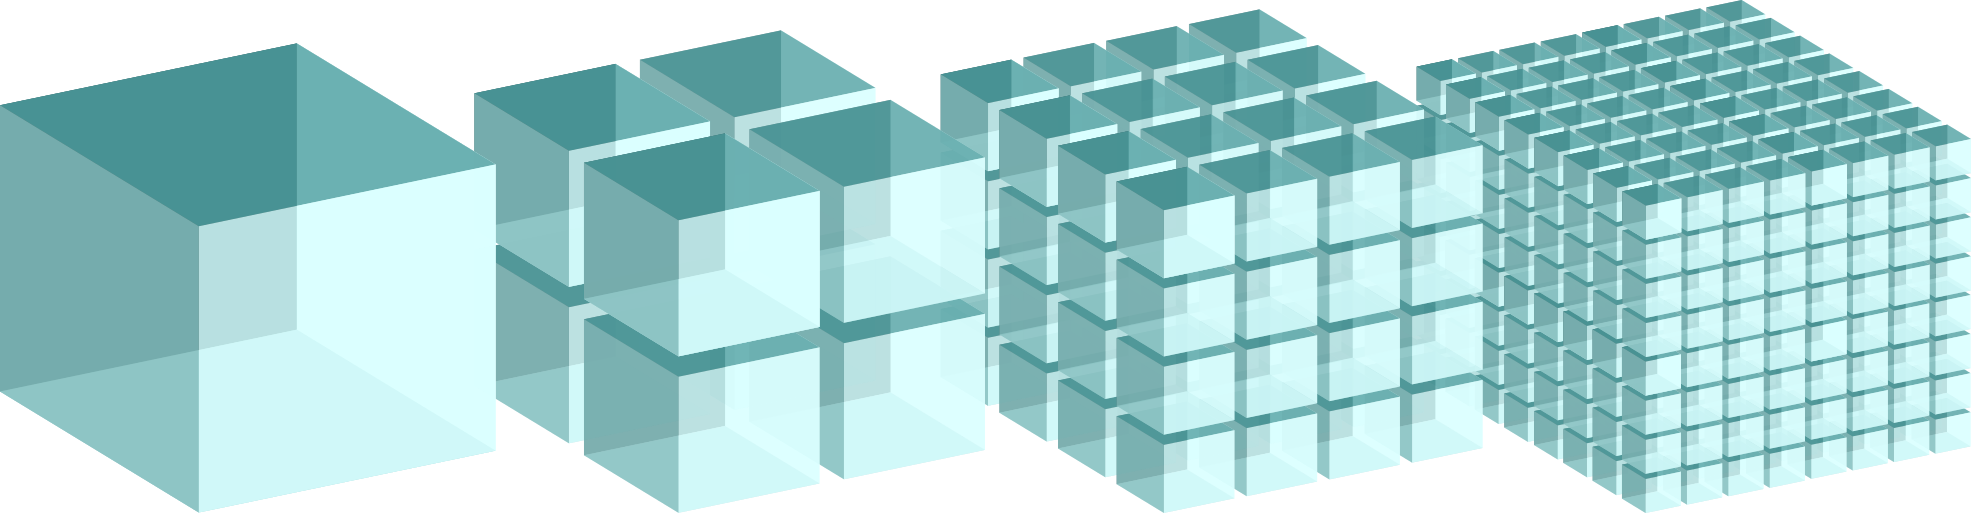
\includegraphics[width=\textwidth]{area_cubes.png}
		}
	
	\caption[Subdivisiones de un cubo demostrando el aumento de área superficial total]{Secuencia de divisiones de un cubo conservando el volumen (cantidad de material). Si se comienza con un cubo de 1 cm de lado y se subdivide hasta tener cubos de 100 nm de lado, el área superficial total pasaría de 6 $\mathrm{cm^2}$ a 60 $\mathrm{m^2}$. En este caso, el lado de un cubo disminuye 100.000 veces, aumentando el área superficial total por el mismo factor.}
	\label{fig:area_cubes}
\end{figure}

\section*{Síntesis de nanomateriales}
Dependiendo de la vía de aproximación a la nanoescala, se distinguen dos formas de síntesis, por un lado, si partimos de la forma macroscópica de un material y de algún modo se reducen sus dimensiones hacia la nanoescala, se habla de un proceso \textit{top-down}. Por ejemplo, la exfoliación del grafito (\textit{bulk material}) para obtener grafeno (nanomaterial) \citep{Novoselov2004}.  Por otro lado, sintetizar un nanomaterial a partir de átomos o moléculas es un proceso \textit{bottom-up}, un ejemplo es la síntesis de nanopartículas de oro a partir de un precursor como el ácido tetracloroaúrico \citep{Daniel2004}.

\section*{Caracterización de nanomateriales}

\chapter{\label{cap:1} Nanonomateriales}

\noindent
\rule{\linewidth}{1 pt}
\begin{flushright}
\begin{quotation}
\small{
\textit{``There’s Plenty of Room at the Bottom.''}}
\end{quotation}
\bf{Richard Feymann}
\end{flushright}
\noindent
\rule{\linewidth}{1 pt}\\
\vspace{1cm}


\section{Nanomateriales}
En un nanomaterial\index{nanomaterial} al menos una de sus dimensiones está en la escala nanométrica. En una mejor definición, hablamos de nanomateriales cuándo alguna de sus dimensiones es menor a alguna de sus longitudes características\index{longitud característica}, dando lugar a la aparición de propiedades diferentes a las de su contraparte macrométrica (bulk material). Los nanomateriales pueden clasificarse por el número de dimensiones en escala nanométrica, con una dimensión constreñida a nanoescala hablamos de materiales 2-dimensionales, pues dos dimensiones están en la macroescala, análogamente, con dos a nanoescala tenemos un material 1-dimensional, y con tres dimensiones a nanoescala, es un material 0-dimensional. Ejemplos de nanomateriales: quantum dots,  nanopartículas (0-dimensional); nanotubos, nanohilos, nanovarillas (1-dimensional); grafeno (2-dimensional).

\section{Síntesis}


\section{Caracterización}

\section{Aplicaciones}

\chapter{\label{cap:2}Grafeno}

\noindent
\rule{\linewidth}{1 pt}
\begin{flushright}
\begin{quotation}
\small{
\textit{``What is important about graphene is the new physics it has delivered.''}}
\end{quotation}
\bf{Andre Geim}
\end{flushright}
\noindent
\rule{\linewidth}{1 pt}\\
\vspace{1cm}

En un nanomaterial\index{nanomaterial} al menos una de sus dimensiones está en la escala nanométrica. En una mejor definición, hablamos de nanomateriales cuándo alguna de sus dimensiones es menor a alguna de sus longitudes características\index{longitud característica}, dando lugar a la aparición de propiedades diferentes a las de su contraparte macrométrica (bulk material). Los nanomateriales pueden clasificarse por el número de dimensiones en escala nanométrica, con una dimensión constreñida a nanoescala hablamos de materiales 2-dimensionales, pues dos dimensiones están en la macroescala, análogamente, con dos dimensiones a nanoescala tenemos un material 1-dimensional, y con tres dimensiones a nanoescala, es un material 0-dimensional. Ejemplos de nanomateriales: quantum dots,  nanopartículas (0-dimensional); nanotubos, nanohilos, nanovarillas (1-dimensional); grafeno (2-dimensional).
\chapter{\label{cap:3}Supercondensadores}

\noindent
\rule{\linewidth}{1 pt}
\begin{flushright}
\begin{quotation}
\small{
\textit{``The force is strong with this one.''}}
\end{quotation}
\bf{Darth Vader}
\end{flushright}
\noindent
\rule{\linewidth}{1 pt}\\
\vspace{1cm}

%ENERGY STORAGE
El almacenar energía eléctrica es uno de los mayores problemas a la hora de diseñar sistemas electrónicos tanto móviles como estacionarios, los requerimientos varían de acuerdo a las necesidades de cada uno, en general es un \textit{trade-off} entre densidad de energía (cuánta energía se puede almacenar) y densidad de potencia (que tan rápido puede ser entregada la energía almacenada). Las celdas de combustible (\textit{Fuel Cells}), entregan la mayor densidad de energía, pero son complicadas, mientras que las baterías poseen mayor densidad de potencia, pierden capacidad con los ciclos de carga y descarga. Los supercondensadores van un paso más allá, aumentado la densidad de potencia y aportando mayor vida útil.

\section{El condensador ideal\index{condensador ideal}}
Generalmente un condensador se modela como un par de placas paralelas separadas por un dieléctrico, es definido por su capacitancia, que refleja la capacidad de almacenar energía. Del modelo de placas paralelas se desprende la definición de capacitancia $C$ como la razón entre la magnitud de carga en cada placa $Q$ y el voltaje entre los terminales $V$:

\begin{equation}
	C = \frac{Q}{V}
\end{equation}

Para fines prácticos, el condensador ideal como componente electrónico es modelado por la ecuación que relaciona la corriente con el voltaje, considerando que $i = dq/dt$:

\begin{equation}
	i(t) = C \frac{dv(t)}{dt}
\end{equation}

\begin{figure}[h!]
	\fbox{
		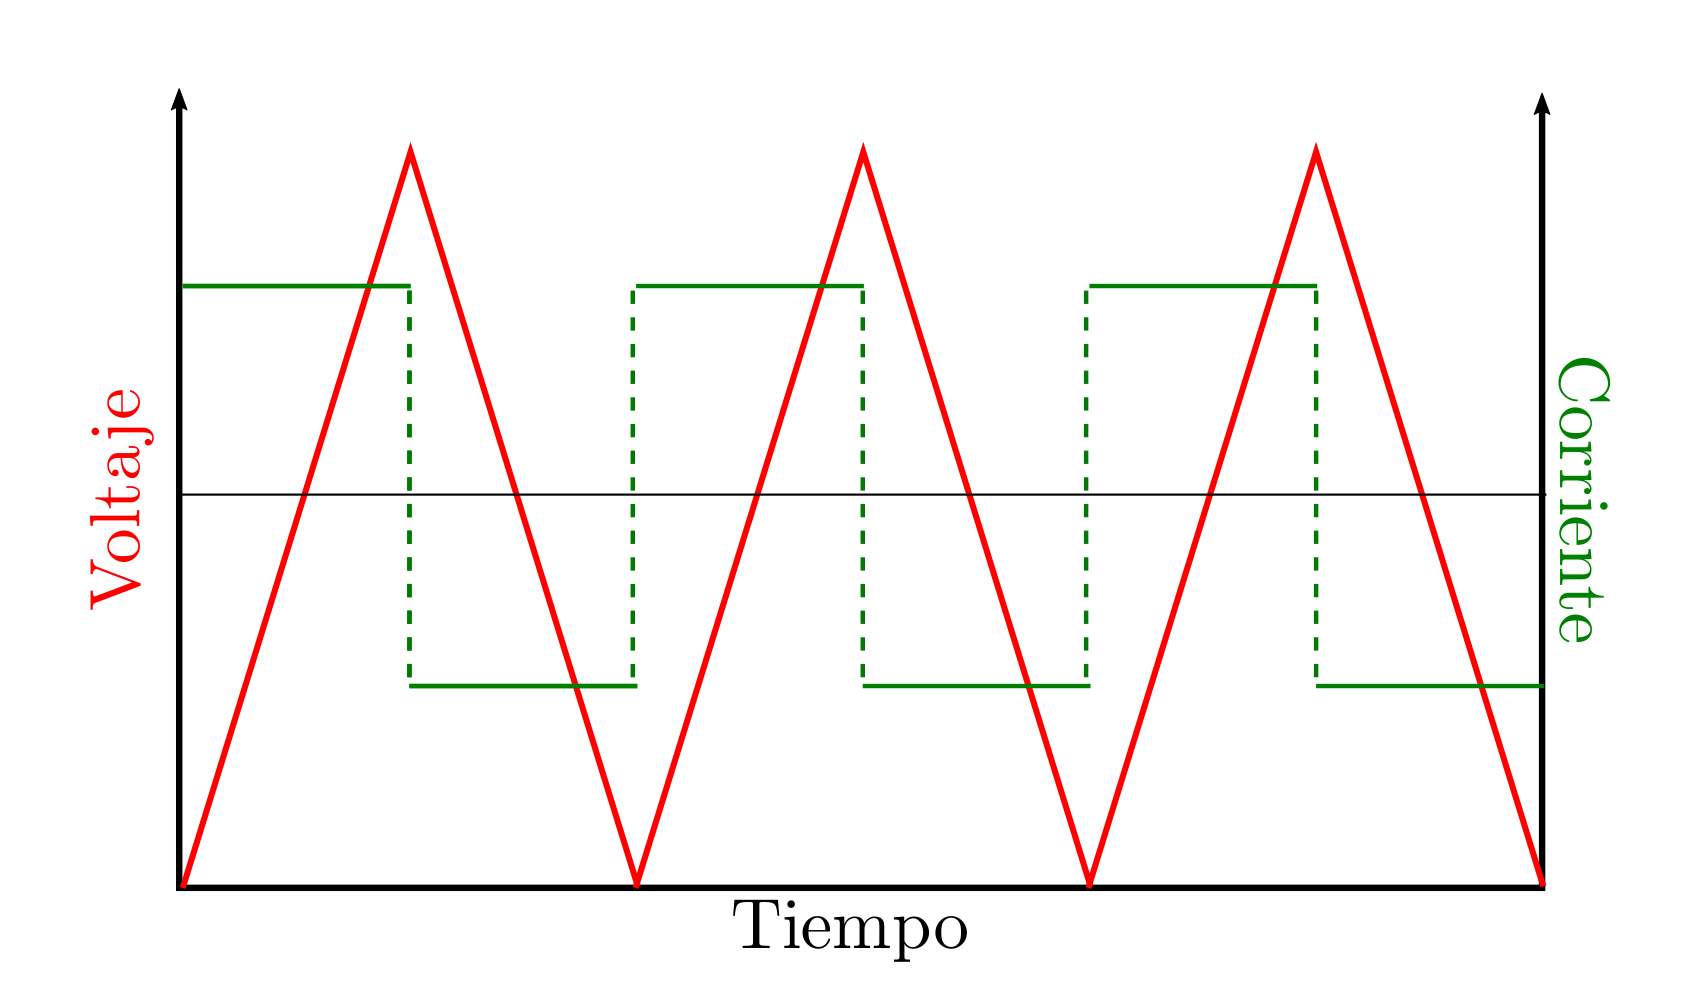
\includegraphics[width=\textwidth]{charge-discharge_ideal_cap.png}
		}
	\caption{Carga y descarga de un condensador ideal a corriente constante.}
	\label{fig:plot:charge-discharge_ideal_cap}
\end{figure}

\section{El condensador real\index{condensador real}}
Un condensador ideal almacenaría energía al cargase y la entregaría al descargarse sin ninguna disipación, es decir, su eficiencia sería del 100\%, podría soportar cualquier voltaje aplicado o cargarse y descargarse por una corriente cuan grande se desee.  En realidad, los condensadores sí disipan energía, poseen voltajes de operación y corrientes máximas de carga y descarga. Todo esto depende de la naturaleza de su construcción y por su puesto, del propósito que fue diseñado.

\subsection{Breakdown voltage}
Los condensadores convencionales construidos con materiales dieléctricos están sujetos a un voltaje máximo de operación determinado por la tensión de ruptura (\textit{Breakdown voltage})\index{tensión de ruptura, \textit{breakdown voltage}}, voltaje al cual se pierden las propiedades dieléctricas del material ocasionando cortocircuito al interior del dispositivo, determinado por la fuerza dieléctrica del material y el espesor de este. En los condensadores electrolíticos la tensión de ruptura es determinada por otros mecanismos\cite{YAHALOM19701429,YAHALOM1971603} que se han mantenido en hipótesis. En lo que respecta a los supercondensadores, el voltaje máximo de carga depende fundamentalmente de electrolíto usado, principalmente por las reacciones que ocurren a ciertos potenciales, este tema será abordado con más detalle en la sección correspondiente.

\subsection{Circuito equivalente}
El comportamiento de los condensadores reales son modeladas por un circuito equivalente, donde se introducen componentes que representan el las imperfecciones del funcionamiento del condensador real.\\
Circuito equivalente\cite{Frackowiak2001937}


\subsubsection{Resistencia en serie equivalente}
Las imperfecciones en la construcción de condensadores, y la naturaleza de los materiales utilizados (e.g. electrodos de resistencia no cero),

\begin{figure}[h!]
	\fbox{
		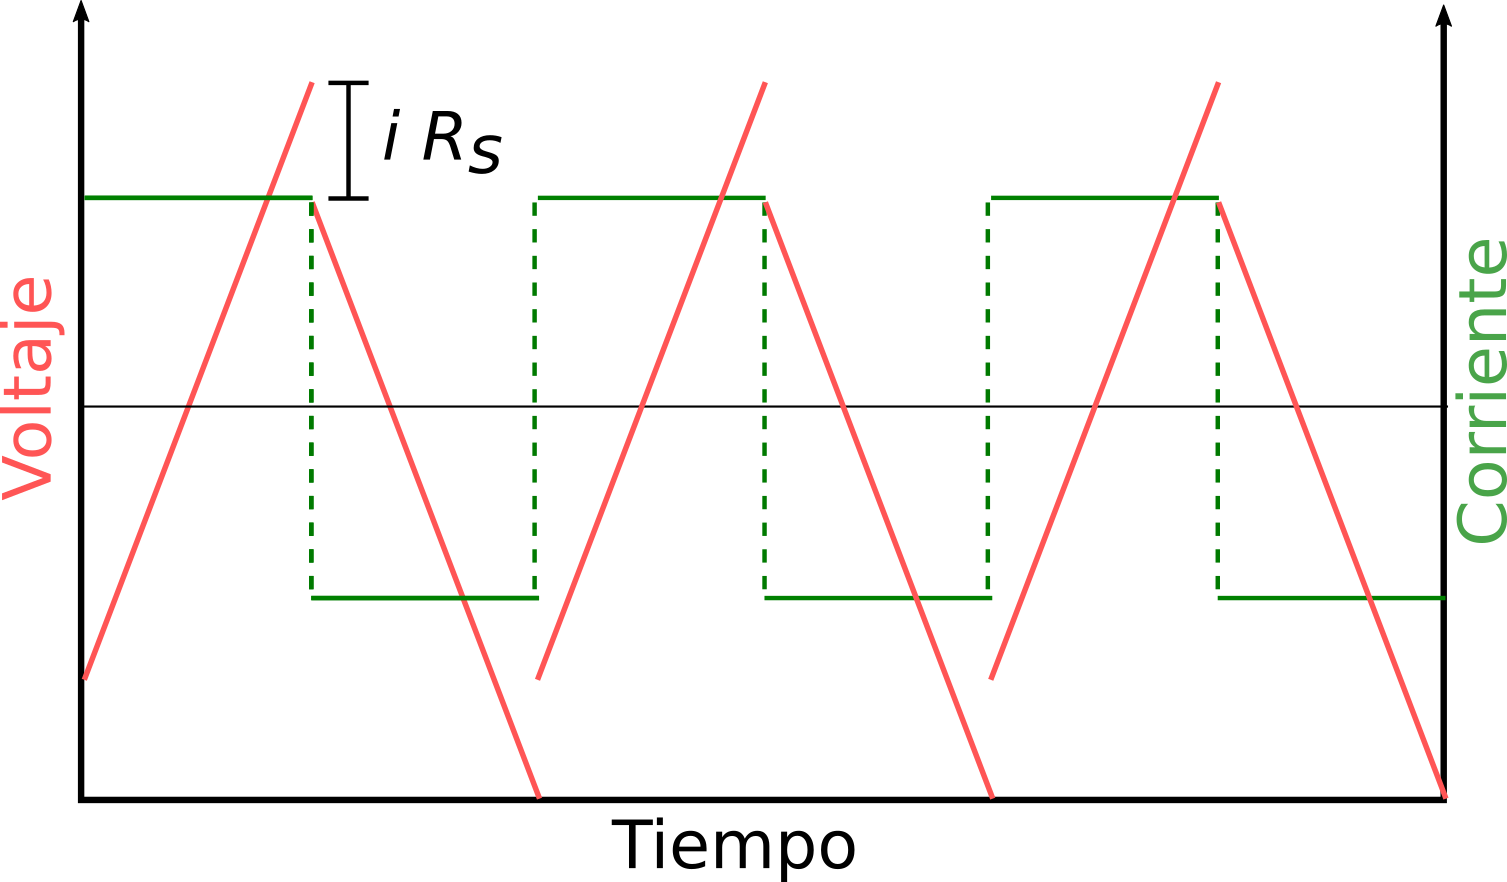
\includegraphics[width=\textwidth]{charge-discharge_esr.png}
	}
	\caption{Carga y d.}
	\label{fig:plot:charge-discharge_esr}
\end{figure}
\section{¿Qué hace a un supercondensador super?}

\subsection{Doble capa electrostática de Helmholtz}

\subsection{Pseudocapacitancia}
\chapter{\label{cap:4}Título Capítulo 4}

\noindent
\rule{\linewidth}{1 pt}
\begin{flushright}
\begin{quotation}
\small{
\textit{Frase célebre}}
\end{quotation}
\bf{Autor}
\end{flushright}
\noindent
\rule{\linewidth}{1 pt}\\
\vspace{1cm}

\chapter{Conclusiones}
%\addcontentsline{toc}{chapter}{Conclusiones}
En este trabajo de tesis se implementó un método efectivo para medir el desempeño de materiales basados en carbono como electrodos de supercondensadores, que resultó ser apropiado para determinar diferencias en la construcción de los electrodos. Además, se sintetizó un material de carbono para ser utilizado como electrodo en dichos condensadores.

Comparando la capacidad específica medida para los electrodos de polvo en sustrato de acero (\mPolvoAcero), y el de polvo en espuma de níquel (\mPolvoNiquel), se observa que el sustrato de acero se desempeña mejor que el de níquel, a pesar de que el sustrato de níquel posee mayor area superficial.

El gráfico de Nyquist revela que los electrodos que exhiben un comportamiento más cercano al esperado para un supercondensador, son las 
muestras de papel y liofilizado.

\chapter*{Anexo}
\addcontentsline{toc}{chapter}{Anexo}

\SCGraphsNoMass{CV_Steel_Disk_No_Material_1}{CV_Steel_Disk_No_Material_2}{0}{16}{1954.91833300000}{Disco de acero sin material.}{200}
\SCGraphs{CV_CRGO300517_9}{CV_CRGO300517_10}{0.0004}{10}{3101.89233300000}{Polvo en disco de acero. Masa = 0.4 mg.}{0.0002}
\SCGraphs{CV_CRGO300517_3}{CV_CRGO300517_4}{0.0028}{20}{2105.33533300000}{Polvo + PMMA en disco de acero. Masa = 2.8 mg.}{0.0002}
\SCGraphs{CV_CRGO300517_11}{CV_CRGO300517_12}{0.0006}{250}{45656.2866670000}{Papel en disco de acero. Masa = 0.6 mg.}{0.0001}
\SCGraphs{CV_CRGO300517_13}{CV_CRGO300517_14}{0.0006}{465}{86333.0367000000}{Material liofilizado en disco de acero. Masa = 0.6 mg.}{0.0001}

\SCGraphsNoMass{CV_Nickel_Foam_No_Material_1}{CV_Nickel_Foam_No_Material_2}{0}{12}{2399.28233300000}{Espuma de níquel sin material.}{200}
\SCGraphs{CV_CRGO300517_5}{CV_CRGO300517_6}{0.0009}{12}{4328.46733300000}{Polvo en espuma de níquel. Masa = 0.9 mg.}{0.0002}
\SCGraphs{CV_CRGO300517_7}{CV_CRGO300517_8}{0.0008}{5}{771.593133000000}{Polvo + PMMA en espuma de níquel. Masa = 0.8 mg.}{0.0002}

%PÁGINAS FINALES

%(1) GLOSARIO (Índice Analítico)	[]
\newpage
\printindex
\addcontentsline{toc}{chapter}{Índice Analítico}	%Para que aparezca en el índice

%(2) BIBLIOGRAFÍA			[]
\newpage
\printbibliography

%(3) ANEXOS(OPTATIVA)			[]
%(4) APÉNDICE(OPTATIVA)			[]
%(5) MATERIAL COMPLEMENTARIO(OPTATIVO)	[]
\end{document}